\chapter{Számítógépes vizsgálatok}\label{ch:futtatas}

Ebben a fejezetben bemutatunk a témához kötődően néhány futtatást, ami szemlélteti \aref{cDMP}. klasszikus diszkrét maximum-elv teljesülését lineáris végeselemekre. Ehhez az egységnégyzeten adott Poisson-egyenletet tekintjük homogén Dirichlet-peremmel. A feladatot különböző nemnegatív forrásfüggényekre oldjuk meg. A megoldás során egyrészt ellenőrizzük a nemnegativitás teljesülését, másrészt vizsgáljuk, hogy kisebb forrásfüggvényekre az eredmény közelebb kerül-e $0$-hoz. A számítások MATLAB programcsomag segítségével készültek.

\section{A feladat leírása}

Keressük az alábbi homogén Dirichlet-feladat végeselemes megoldását, különböző $f \in L^2(\Omega)$ forrásfüggvények mellett, ahol $f \geq 0$:
\begin{equation}\label{dirichlet_problempelda}		
	\left\{
	\begin{aligned}
		-\Delta u &= f,  &&\quad \text{ha } (x,y) \in \Omega \coloneqq (0,1)\times (0,1), \\
		u(x,y) &= 0, & &\quad \text{ha } (x,y) \in \partial\Omega.
	\end{aligned}
	\right.
\end{equation}

\Aref{2dpelda}. pédában bemutatott Courant-elemekkel dolgozunk, azaz a $\mathcal{T}_h$ trianguláció elemei háromszögek,  $u|_{T_k}$ folytonos, szakaszonként lineáris függvény, és a csomóponti értékek a háromszög csúcsaiban vett függvényértékek. A $V_h$ altér ekkor:
\begin{equation*}
	V_h = \left\{ u \in C(\closure{\Omega}): u|_{T_k} \in P^1, \forall T_k \in \mathcal{T}_h, \text{ és } u|_{ \partial \Omega} = 0 \right\}.
\end{equation*}	
A $V_h$ altér bázisát (a síkbeli belső csomópontokat $(x_i,y_j)$-vel jelölve) a szokásos $\varphi_{ij}(x_k,y_l) = \delta_{ik} \cdot \delta_{jl}$ feltétel alapján meghatározott sátorfüggvények alkotják (\ref{fig:2dlinearis} ábra).

Mivel \aref({dirichlet_problempelda}) feladatban $q \equiv 0$, ezért \aref{cDMP_telj}. állítás és \aref{2dszogfelt}. megjegyzés miatt a \aref{cDMP}. klasszikus diszkrét maximum-elv teljesül a feladatra, ha a háromszögrácsban minden $\alpha$ belső szögre $\alpha \leq \pi/2$ teljesül, és $h$ elegendően kicsi, ezért alkalmazzunk szabályos háromszögrácsot. A szabályos háromszögrácsot négyzetrácsból származtatjuk úgy, hogy a négyzeteket az ugyanolyan irányú átlóival daraboljuk. A rács belső osztóponjainak számát $n$ jelöli.

A források legyenek a következő $L^2(\Omega)$-beli nemnegatív függvények:
\begin{equation}\label{f_ek_szamitashoz}
	\begin{aligned}
	f_1 &\equiv 1, \\
	f_{2,k} &= \begin{cases} 1, &\quad  x \leq k \\  0, &\quad \text{különben} \end{cases} 	\\
	f_{3,k} &= \begin{cases} 1, &\quad  x \leq k \text{ vagy } x \geq 1-k  \text{ vagy }\\
								&\quad y \leq k \text{ vagy } y \geq 1-k,\\  
							 0, &\quad \text{különben}\end{cases} 		\\
	f_{4,k} &= \begin{cases} 1, &\quad k \leq x, y \leq 1-k \\  0, &\quad \text{különben}\end{cases} 		
	\end{aligned}
\end{equation}



A belső osztópontok száma legyen $n = 30$, és számítsuk ki \aref({dirichlet_problempelda}) feladat $u_h$ végeselemes megoldását $f_1, f_{2,k}, f_{3,k}, f_{4,k}$ \eqref{f_ek_szamitashoz}  források és adott $k$ paraméterek  mellett. Alkalmazzuk a $k = 1/2, 1/3, 1/5$ paraméterértékeket az $f_{2,k}$ forrásfüggvénynél, és a $k = 1/3, 1/5$ paraméterértékeket az $ f_{3,k}, f_{4,k}$ források esetén. Ekkor az eredményeket \aref{fig:f12eredmeny} és \ref{fig:f34eredmeny} ábrák szemléltetik. A számítások sorrán futtatott MATLAB kódokat mellékeltem \aref{fuggelek}ben. 

\section{Az eredmények értékelése}

\begin{figure}[ht]
	% \centering
	\begin{subfigure}{.5\textwidth}
		\centerline{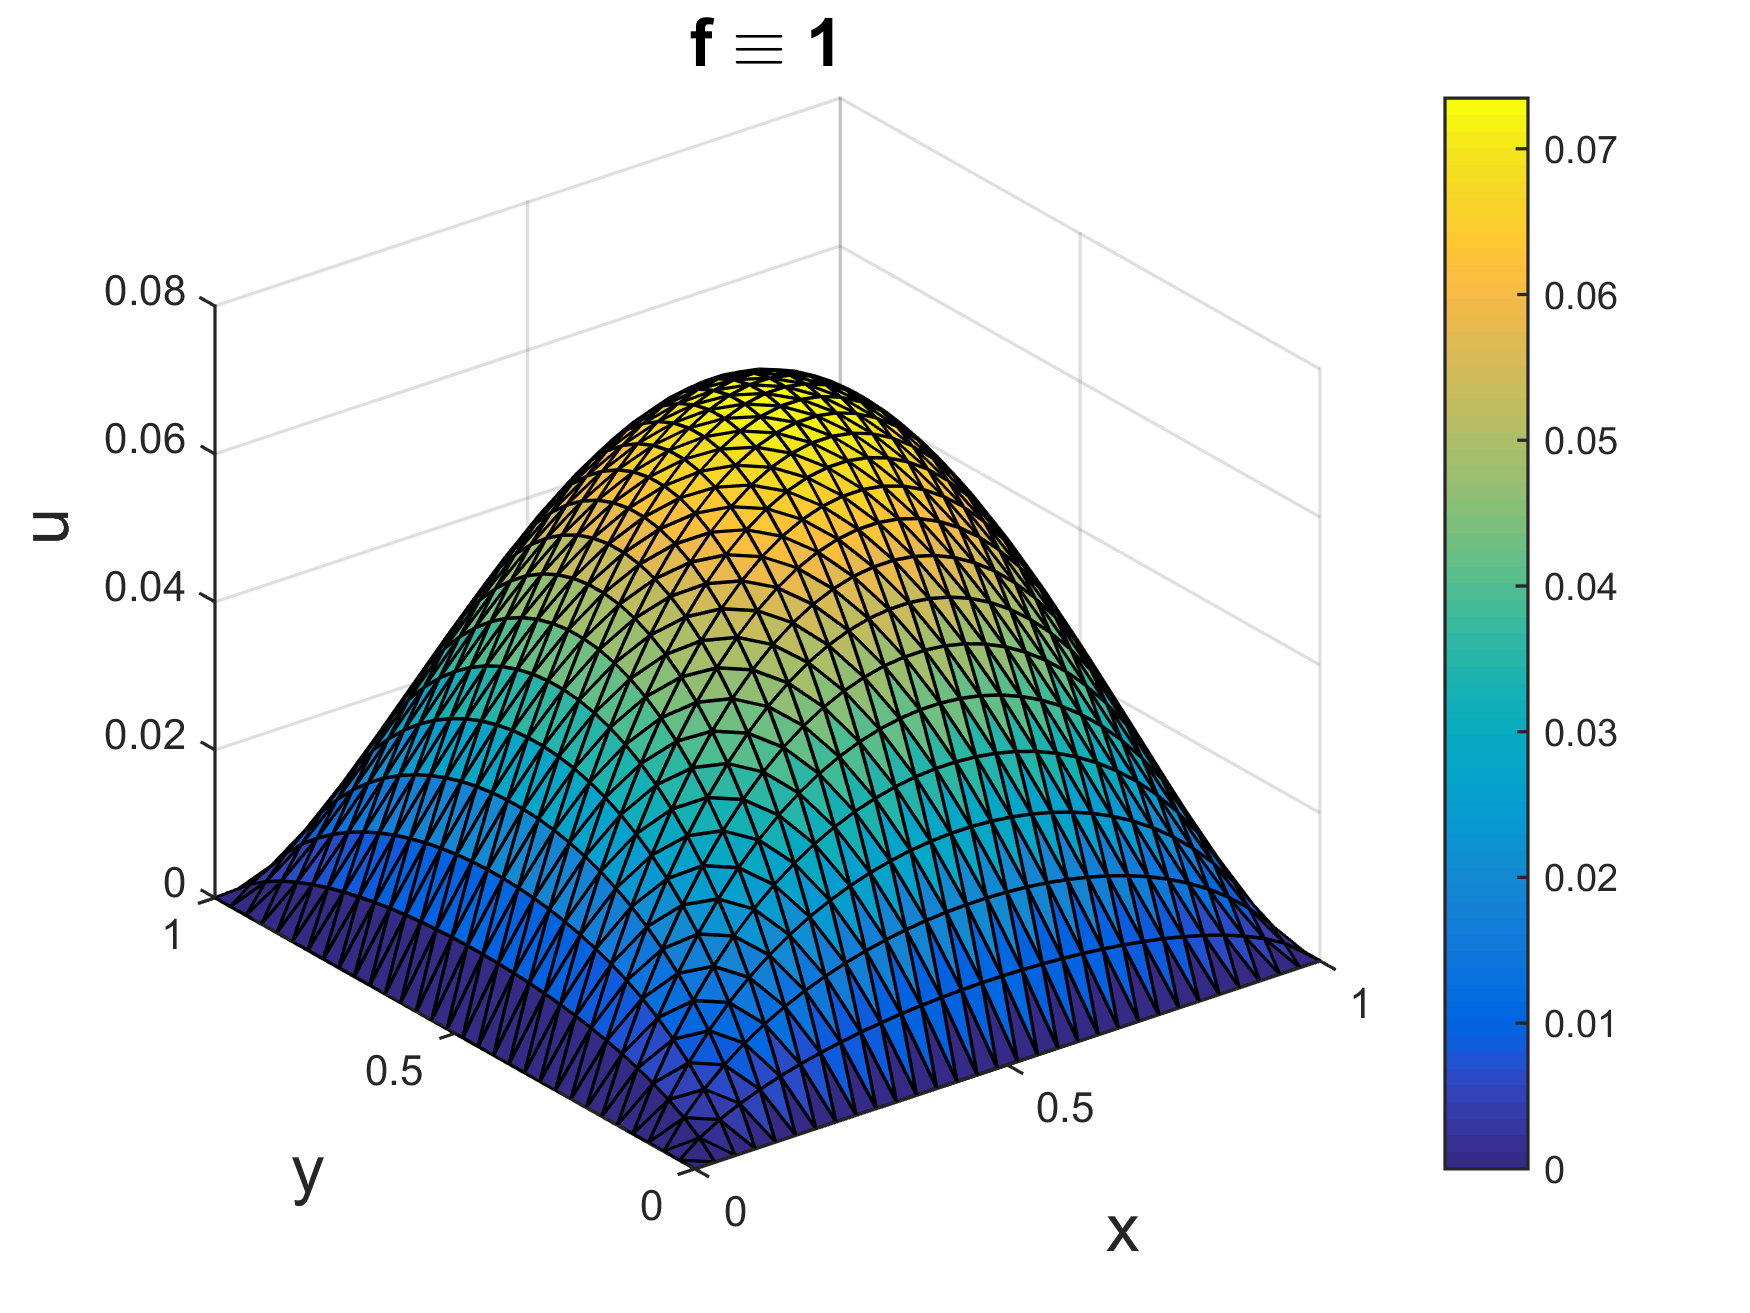
\includegraphics[width=\textwidth]{const100.png}}
		\label{fig:linu2d}
	\end{subfigure}
	~
	\begin{subfigure}{.5\textwidth}
		\centerline{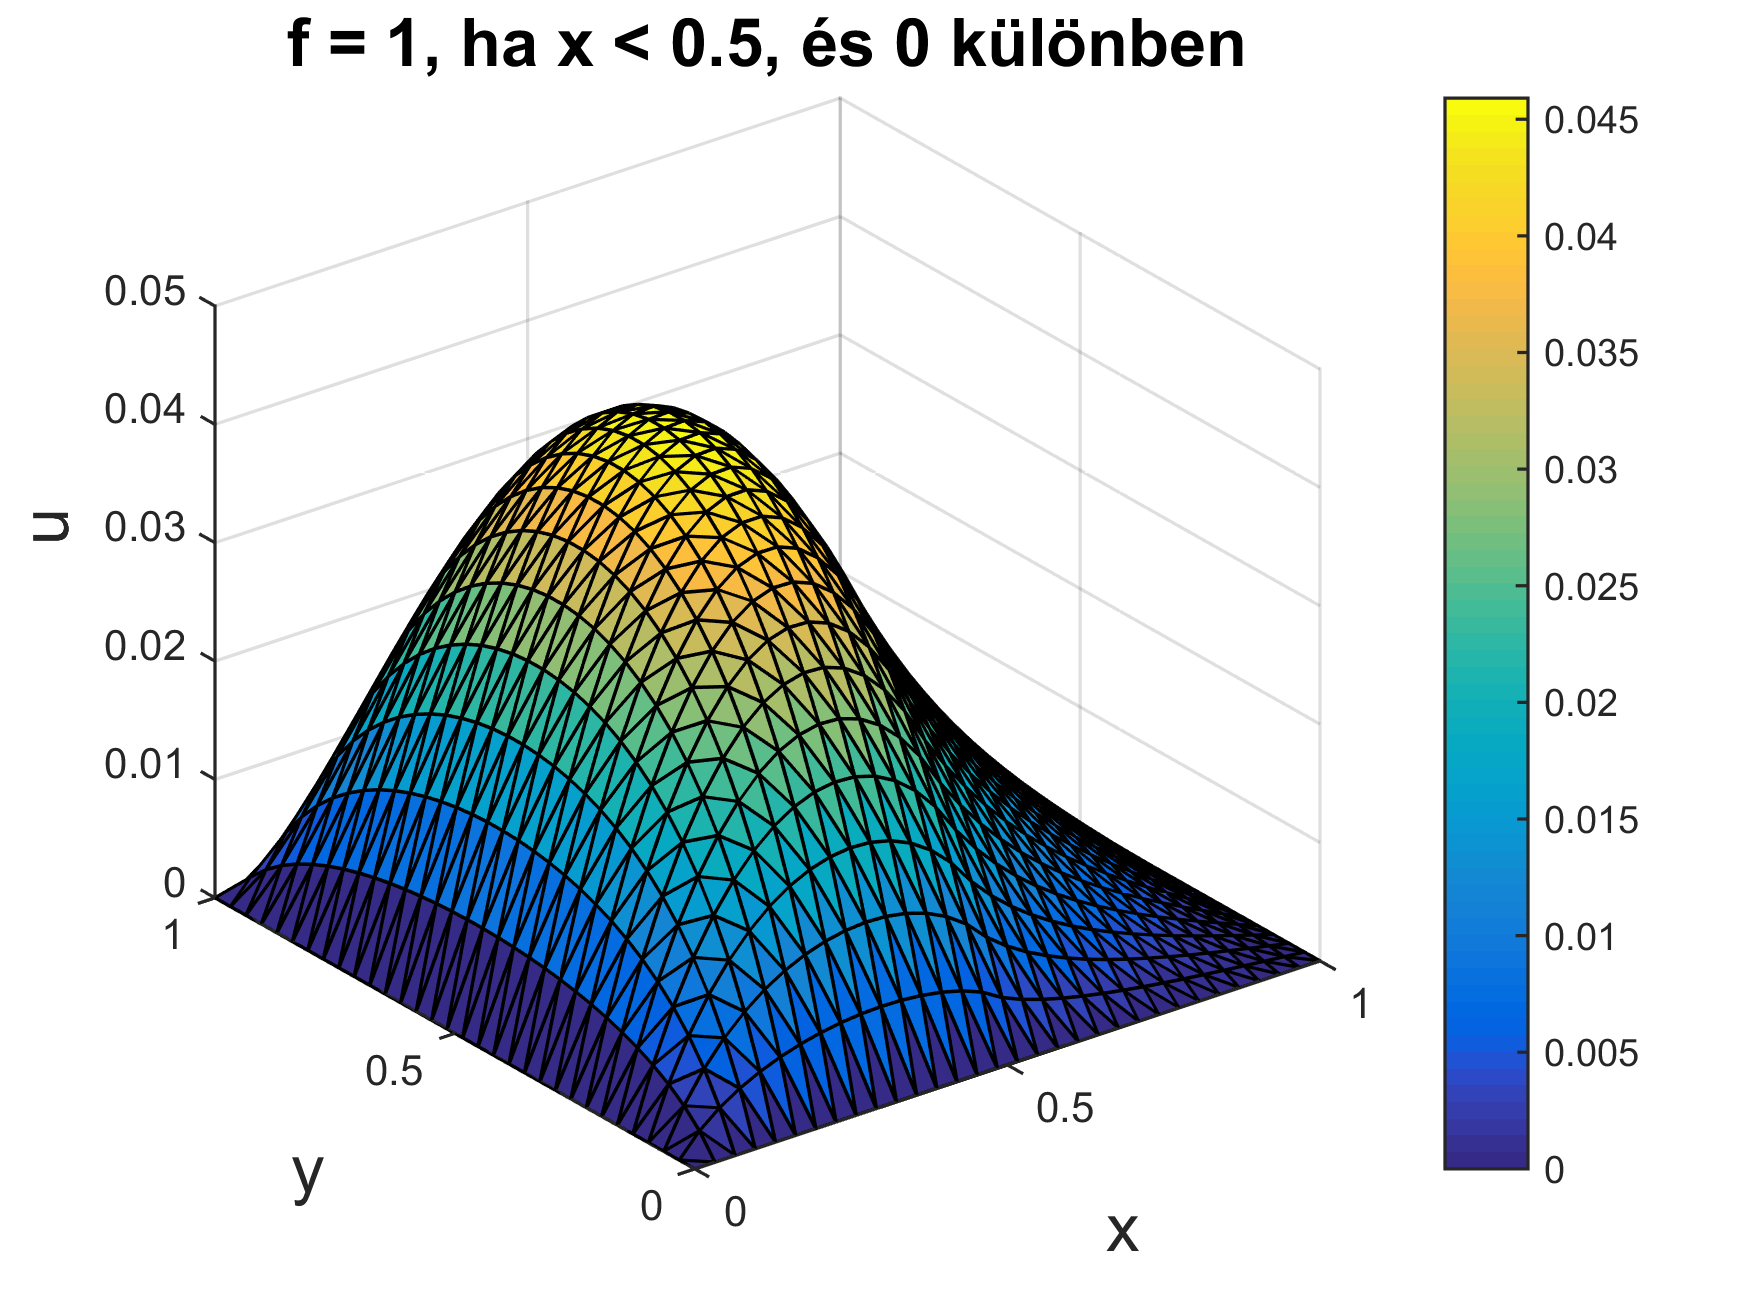
\includegraphics[width=\textwidth]{leftside50.png}}
		\label{fig:linu2d}
	\end{subfigure}
	\\
	\begin{subfigure}{.5\textwidth}
		\centerline{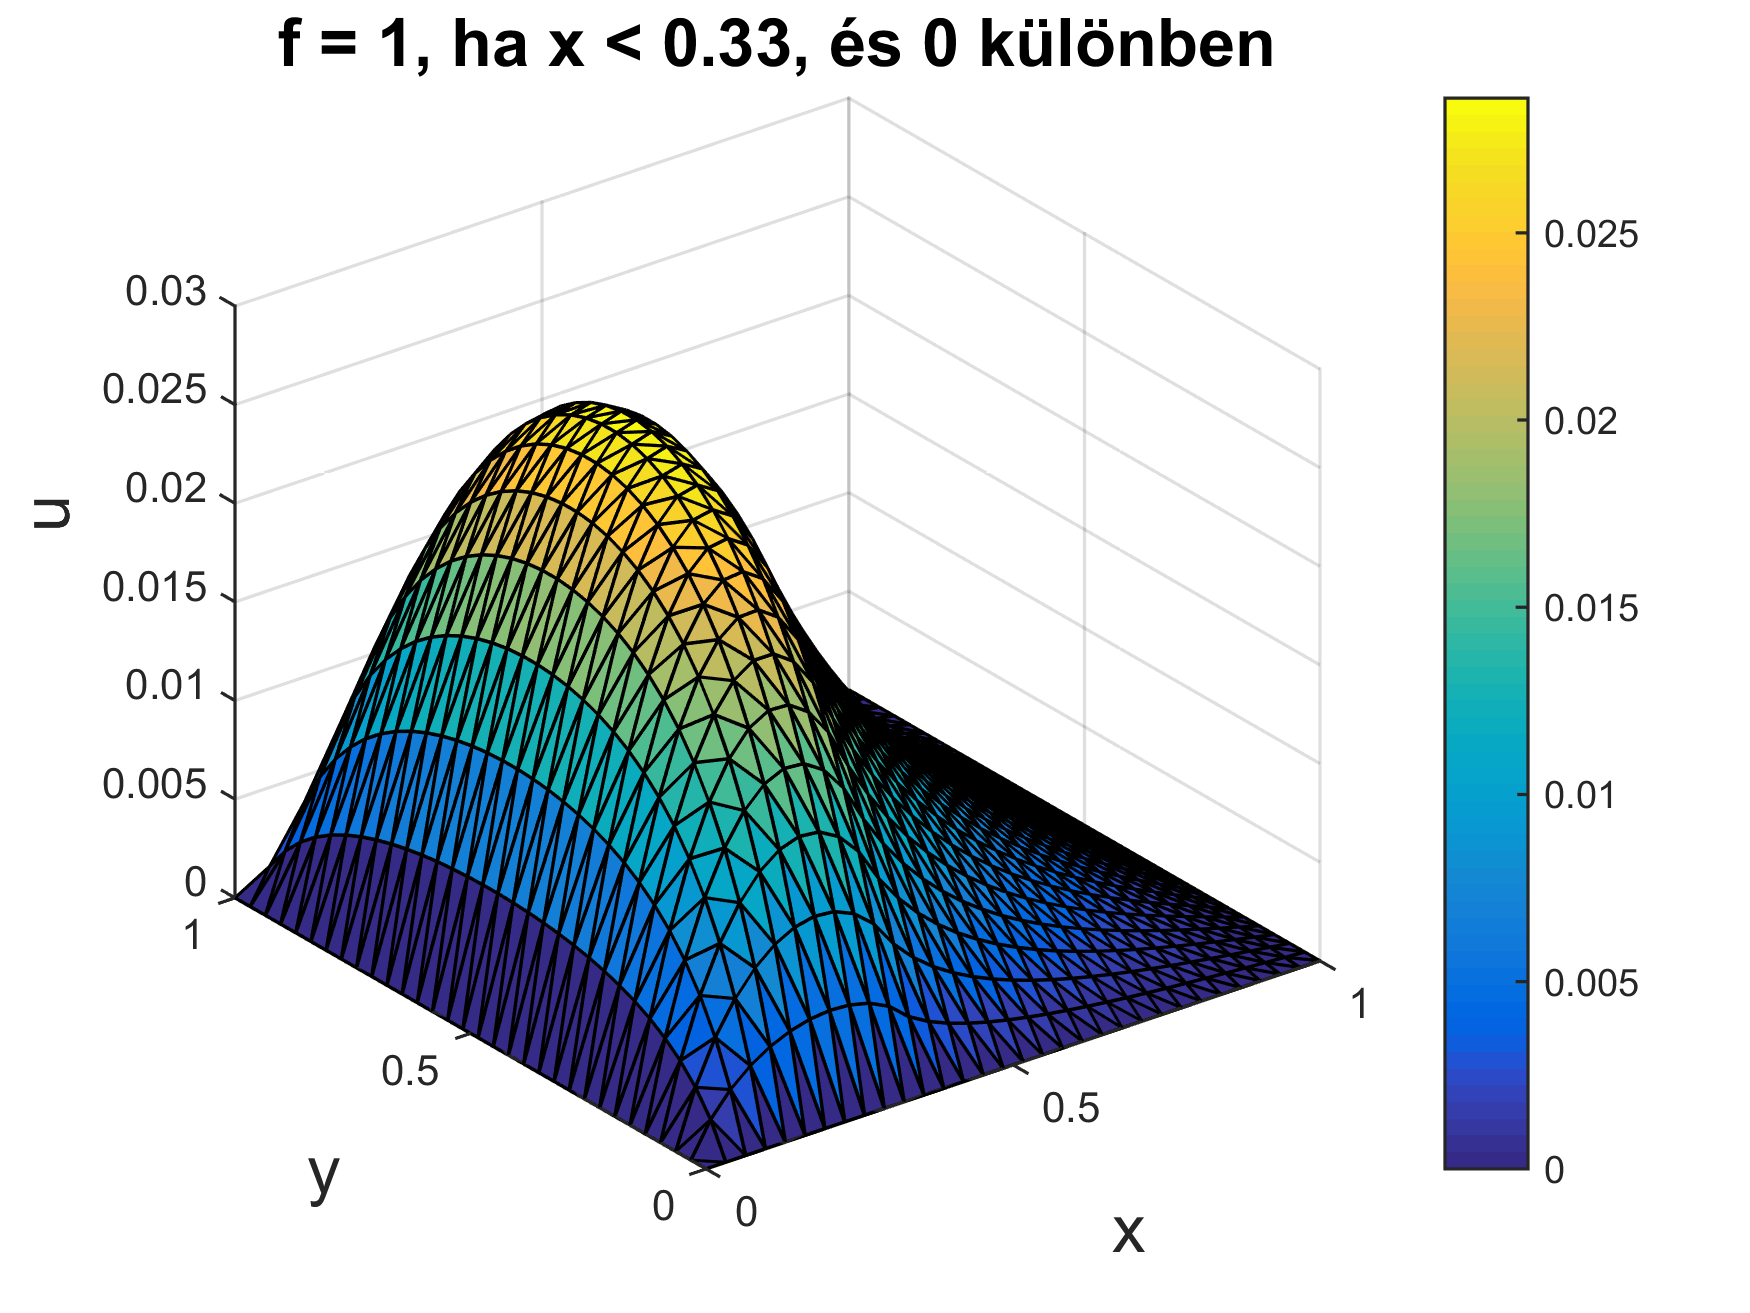
\includegraphics[width=\textwidth]{leftside33.png}}
		\label{fig:linu2d}
	\end{subfigure}
	~
	\begin{subfigure}{.5\textwidth}
		\centerline{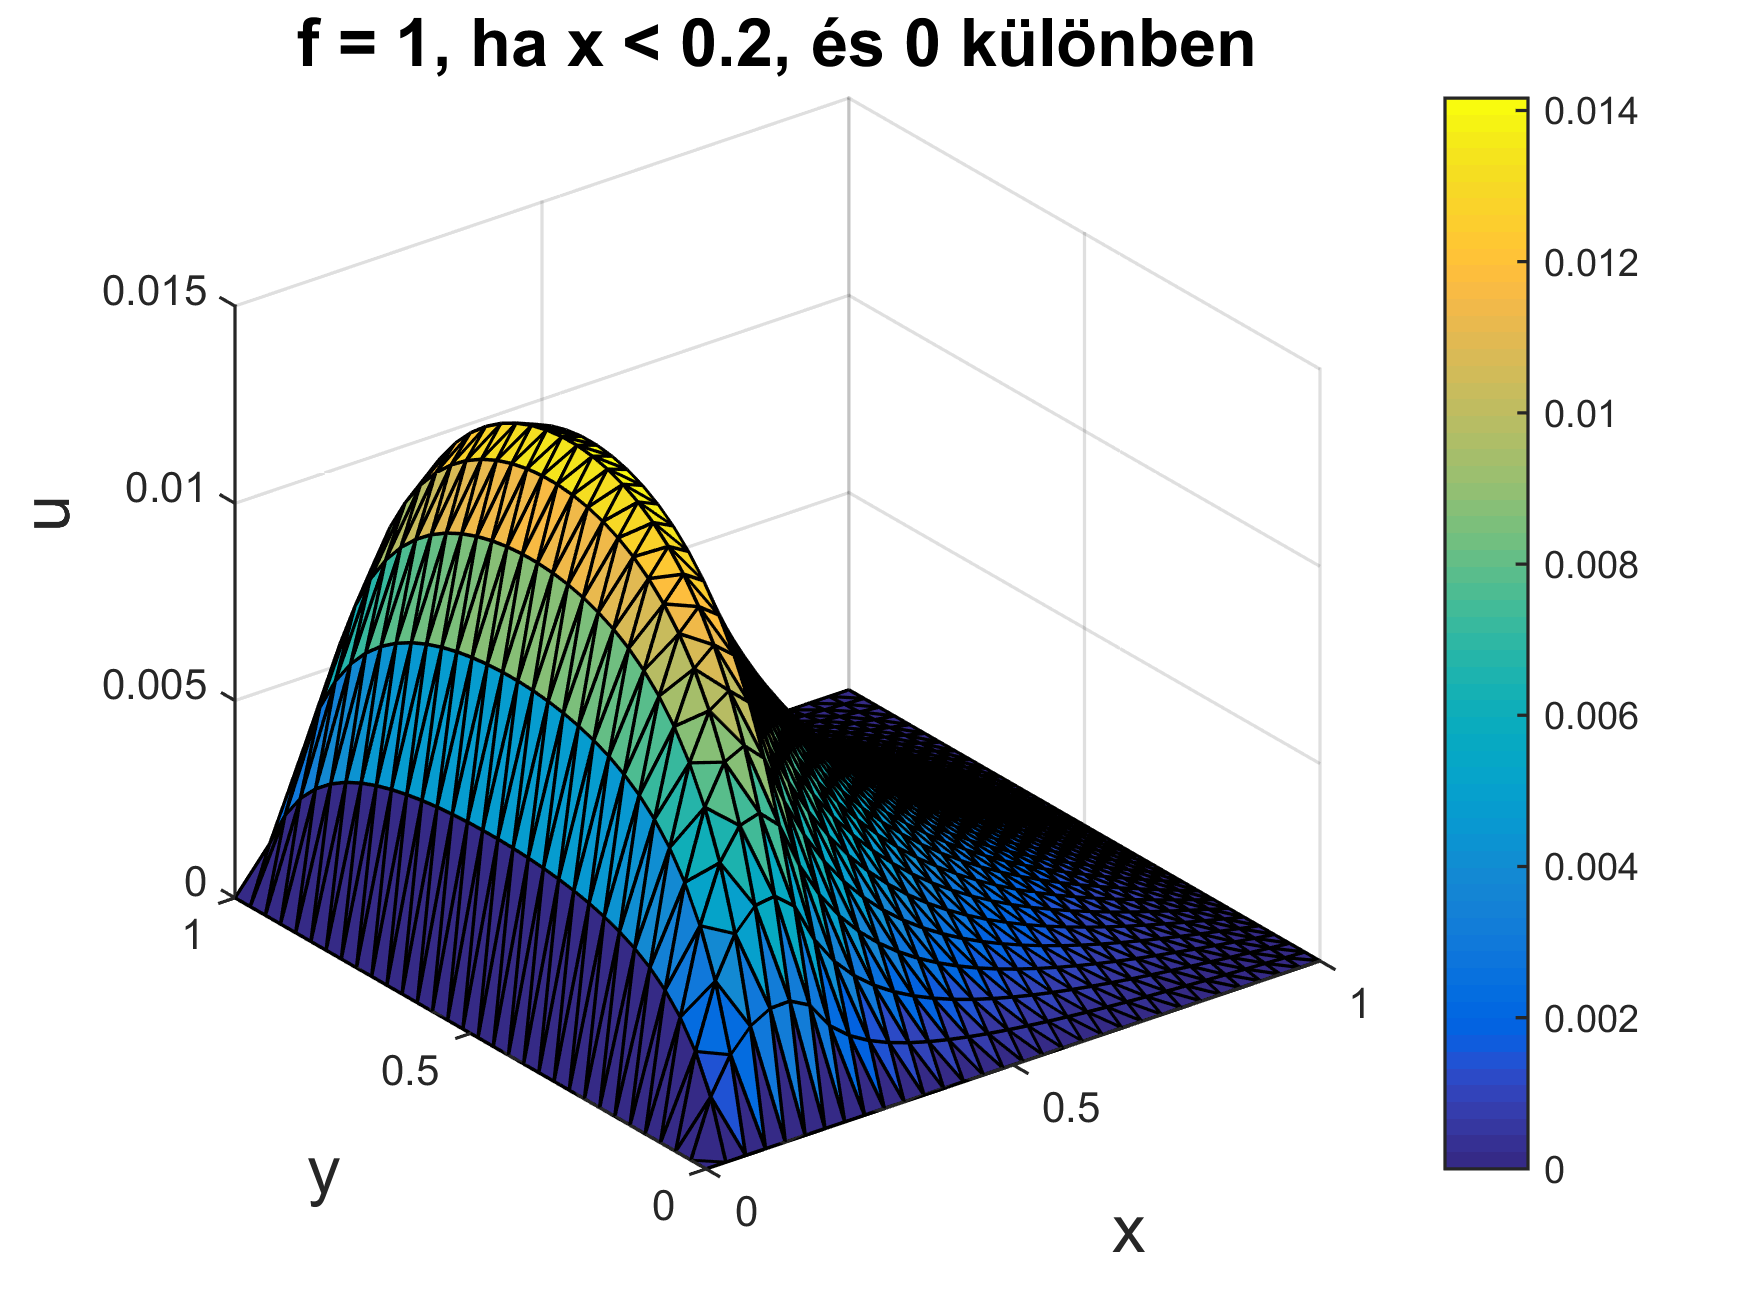
\includegraphics[width=\textwidth]{leftside20.png}}
		\label{fig:linu2d}
	\end{subfigure}
	\caption{Eredmények az $f_1$, illetve és $f_{2,k}$ jobb oldali függvényekre \eqref{f_ek_szamitashoz}, $k = 1/2, 1/3, 1/5$ mellett.}
	\label{fig:f12eredmeny}
\end{figure}

\begin{figure}[ht]
	% \centering
	\begin{subfigure}{.5\textwidth}
		\centerline{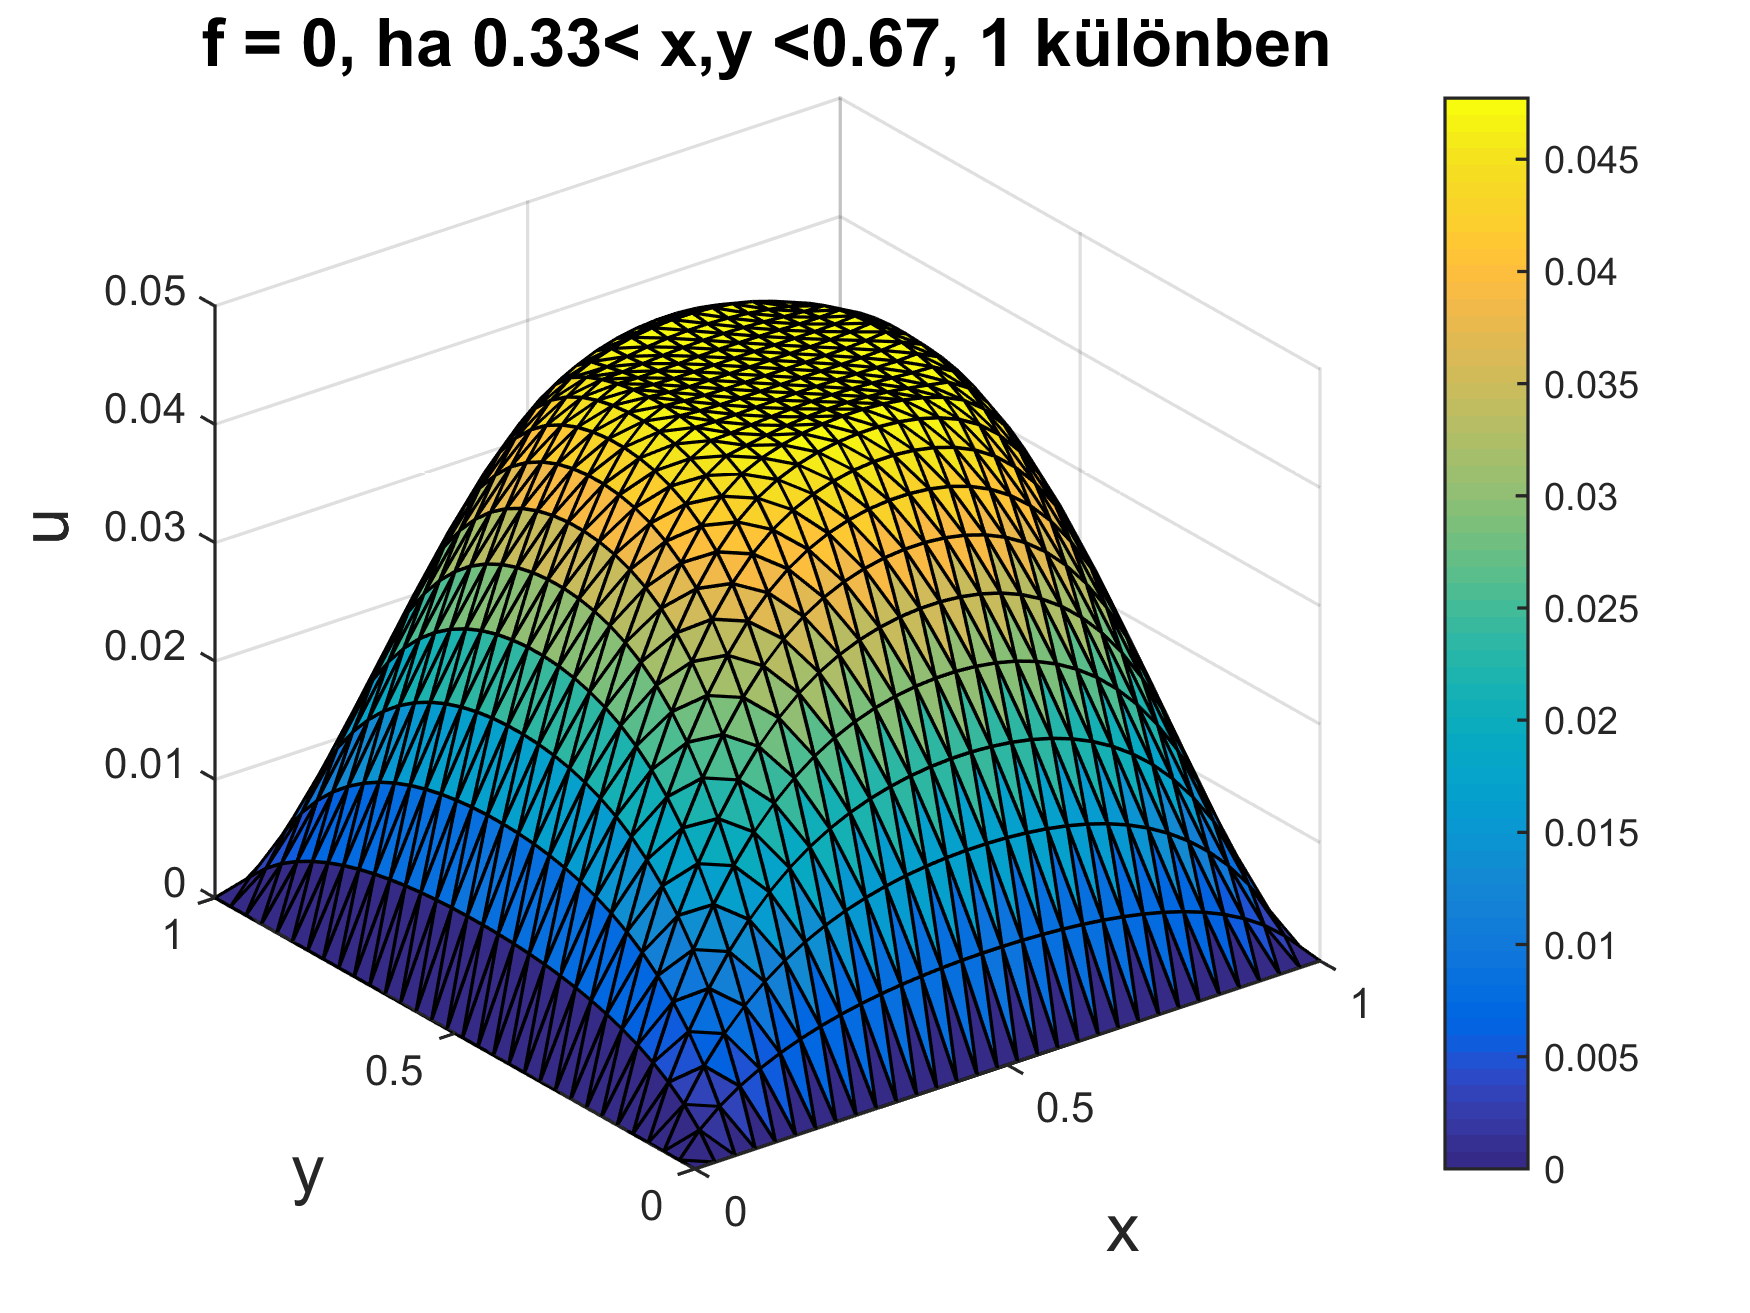
\includegraphics[width=\textwidth]{edge33.png}}
		\label{fig:linu2d}
	\end{subfigure}
	~
	\begin{subfigure}{.5\textwidth}
		\centerline{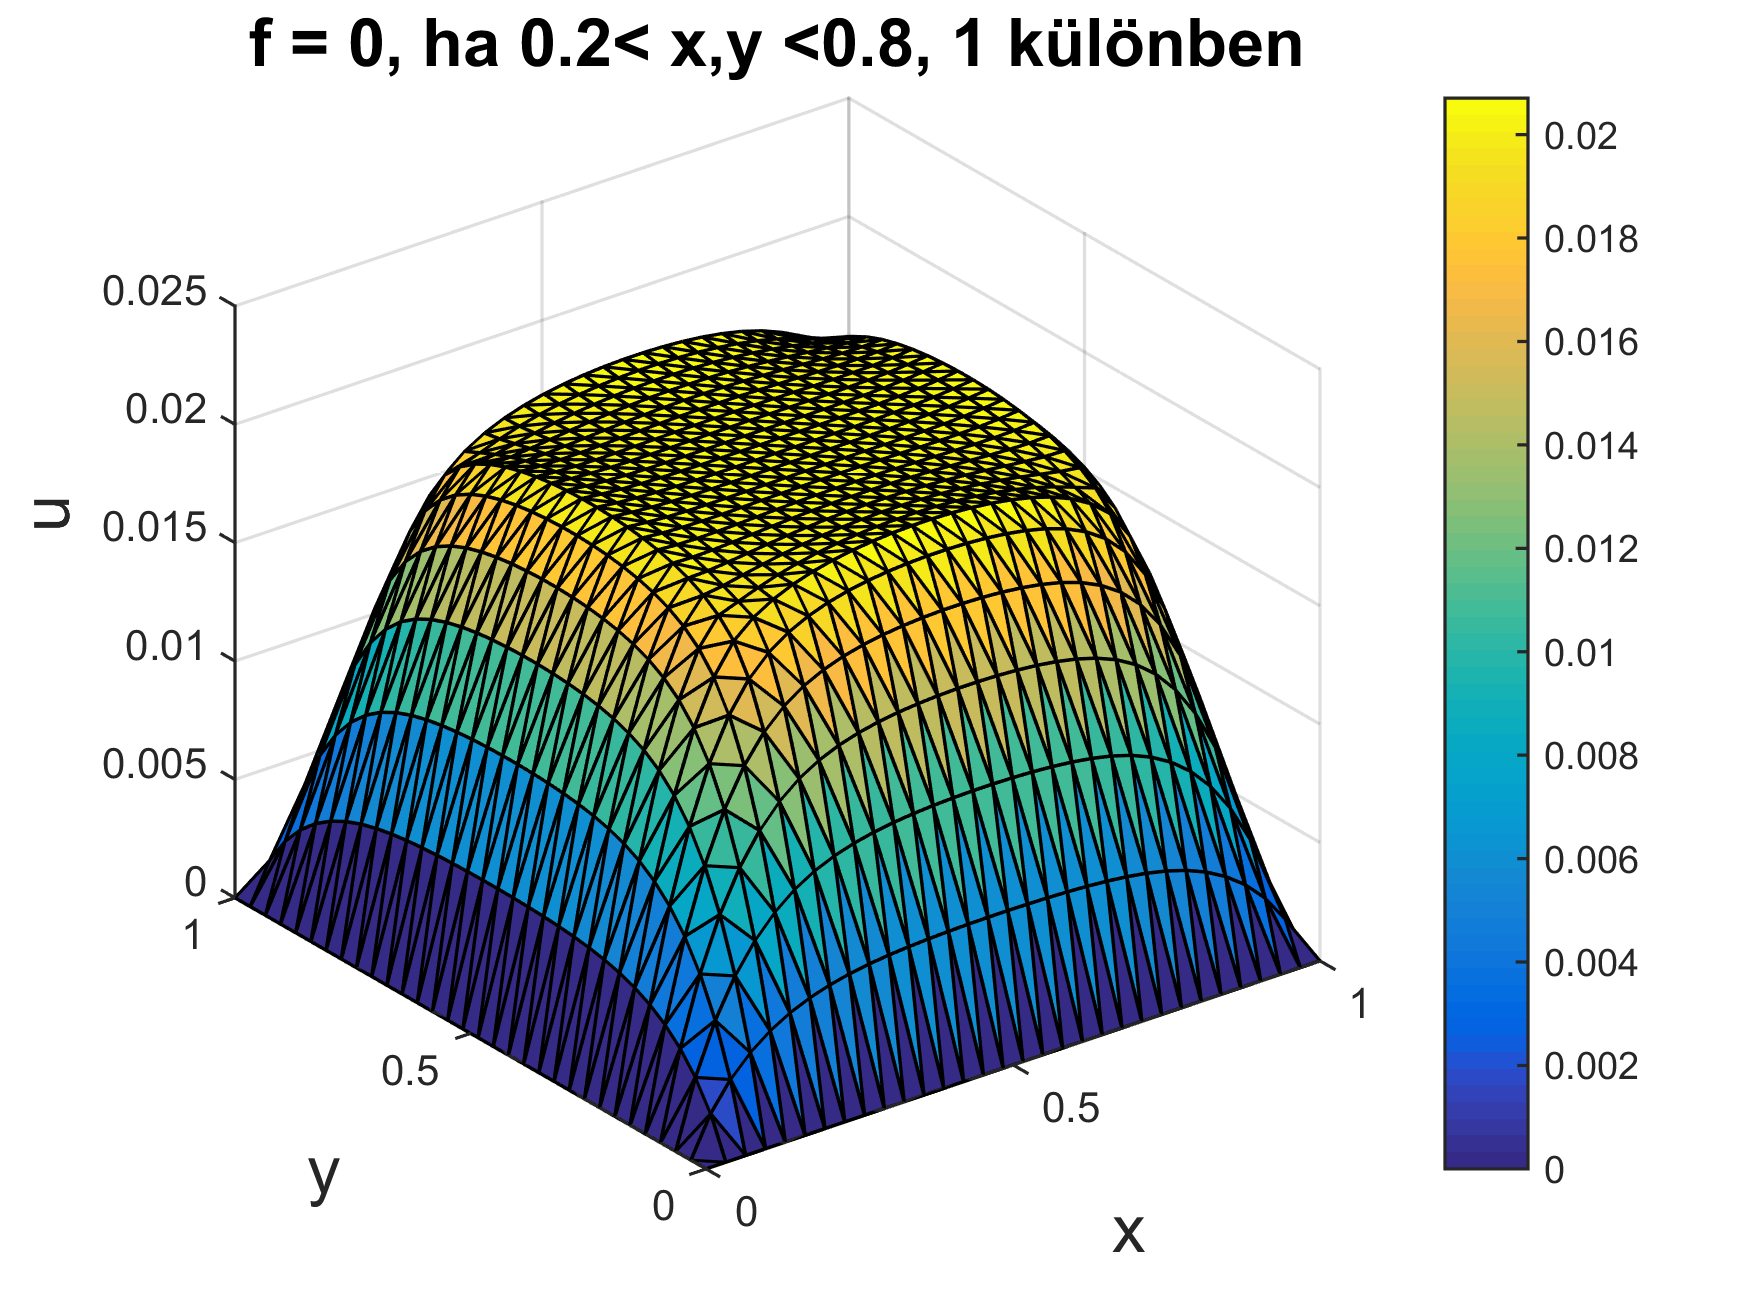
\includegraphics[width=\textwidth]{edge20.png}}
		\label{fig:linu2d}
	\end{subfigure}
	\\
	\begin{subfigure}{.5\textwidth}
		\centerline{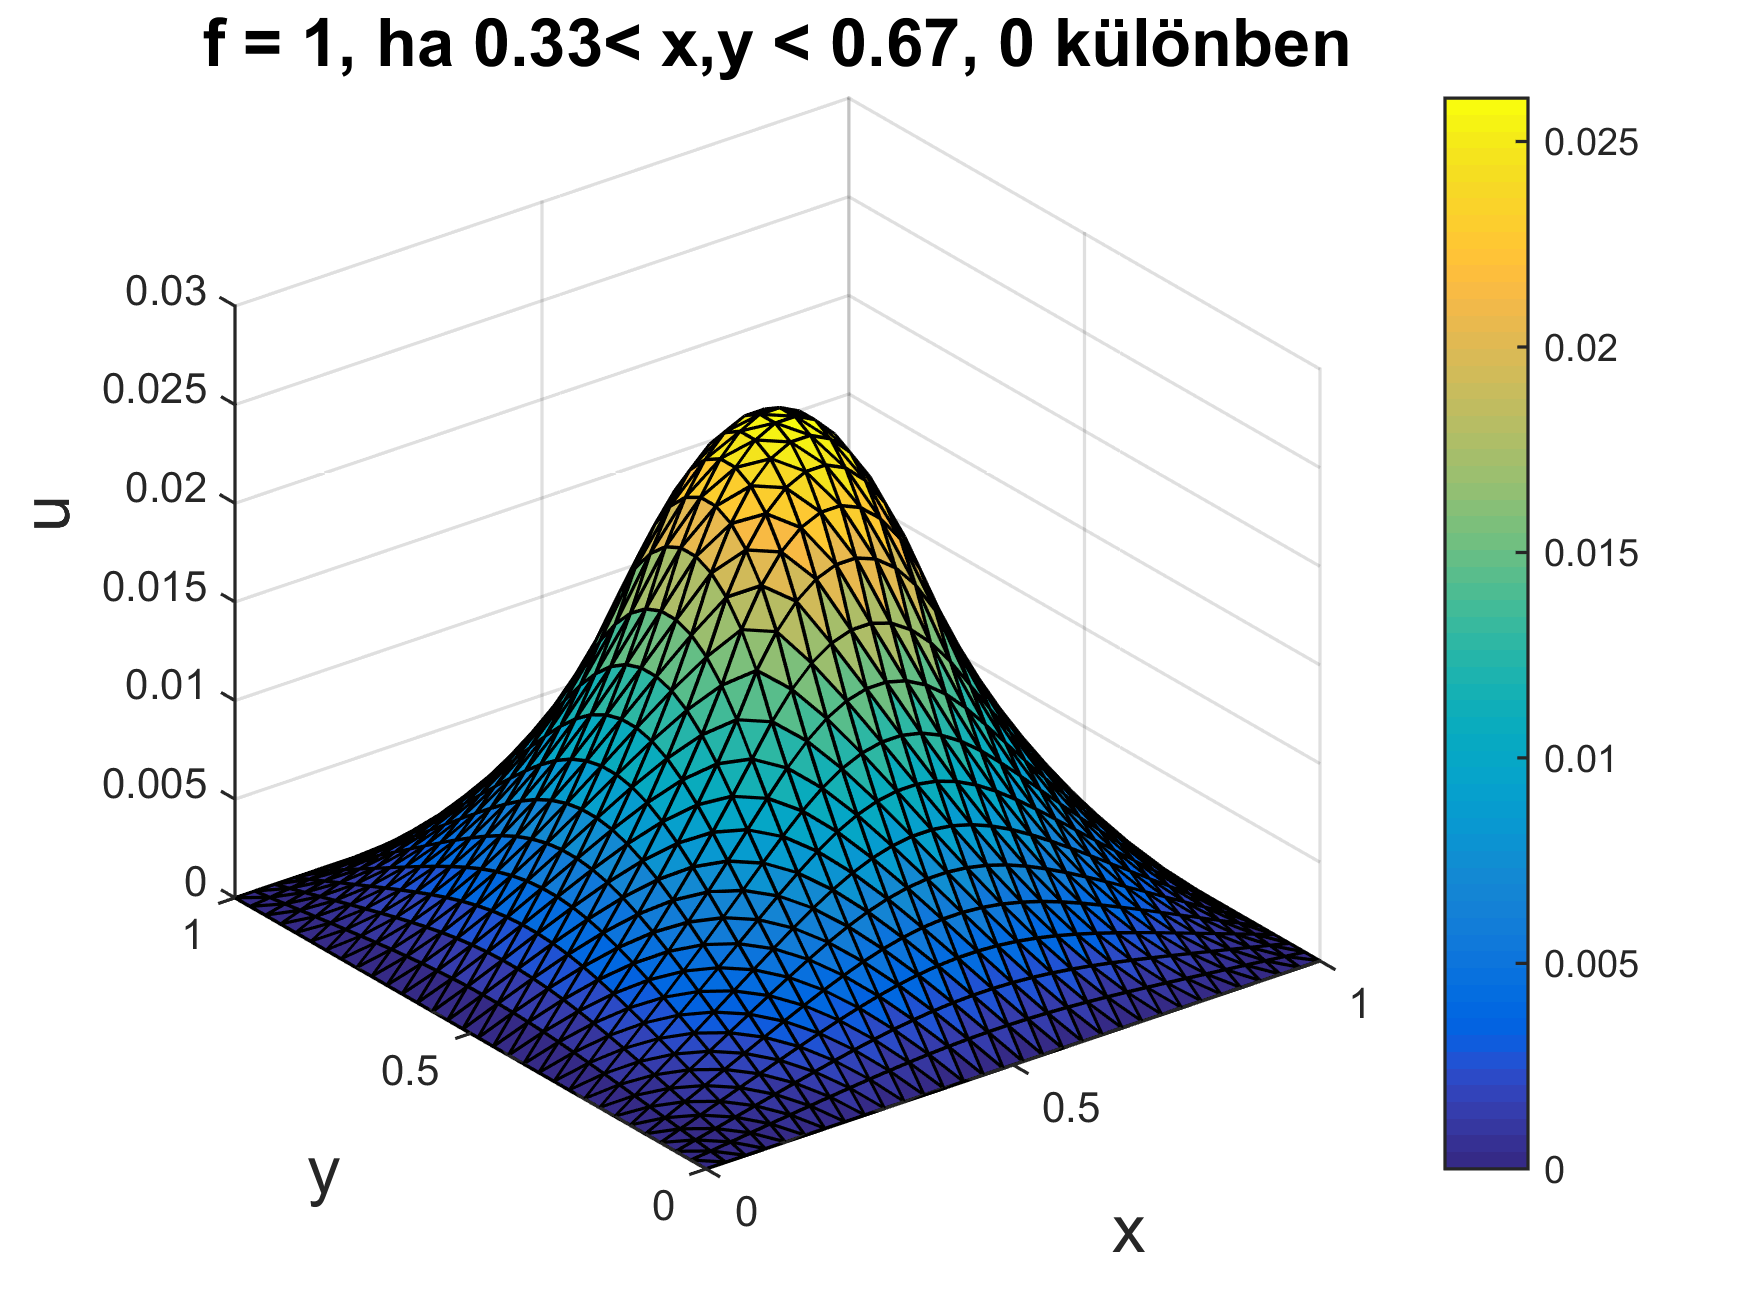
\includegraphics[width=\textwidth]{center33.png}}
		\label{fig:linu2d}
	\end{subfigure}
	~
	\begin{subfigure}{.5\textwidth}
		\centerline{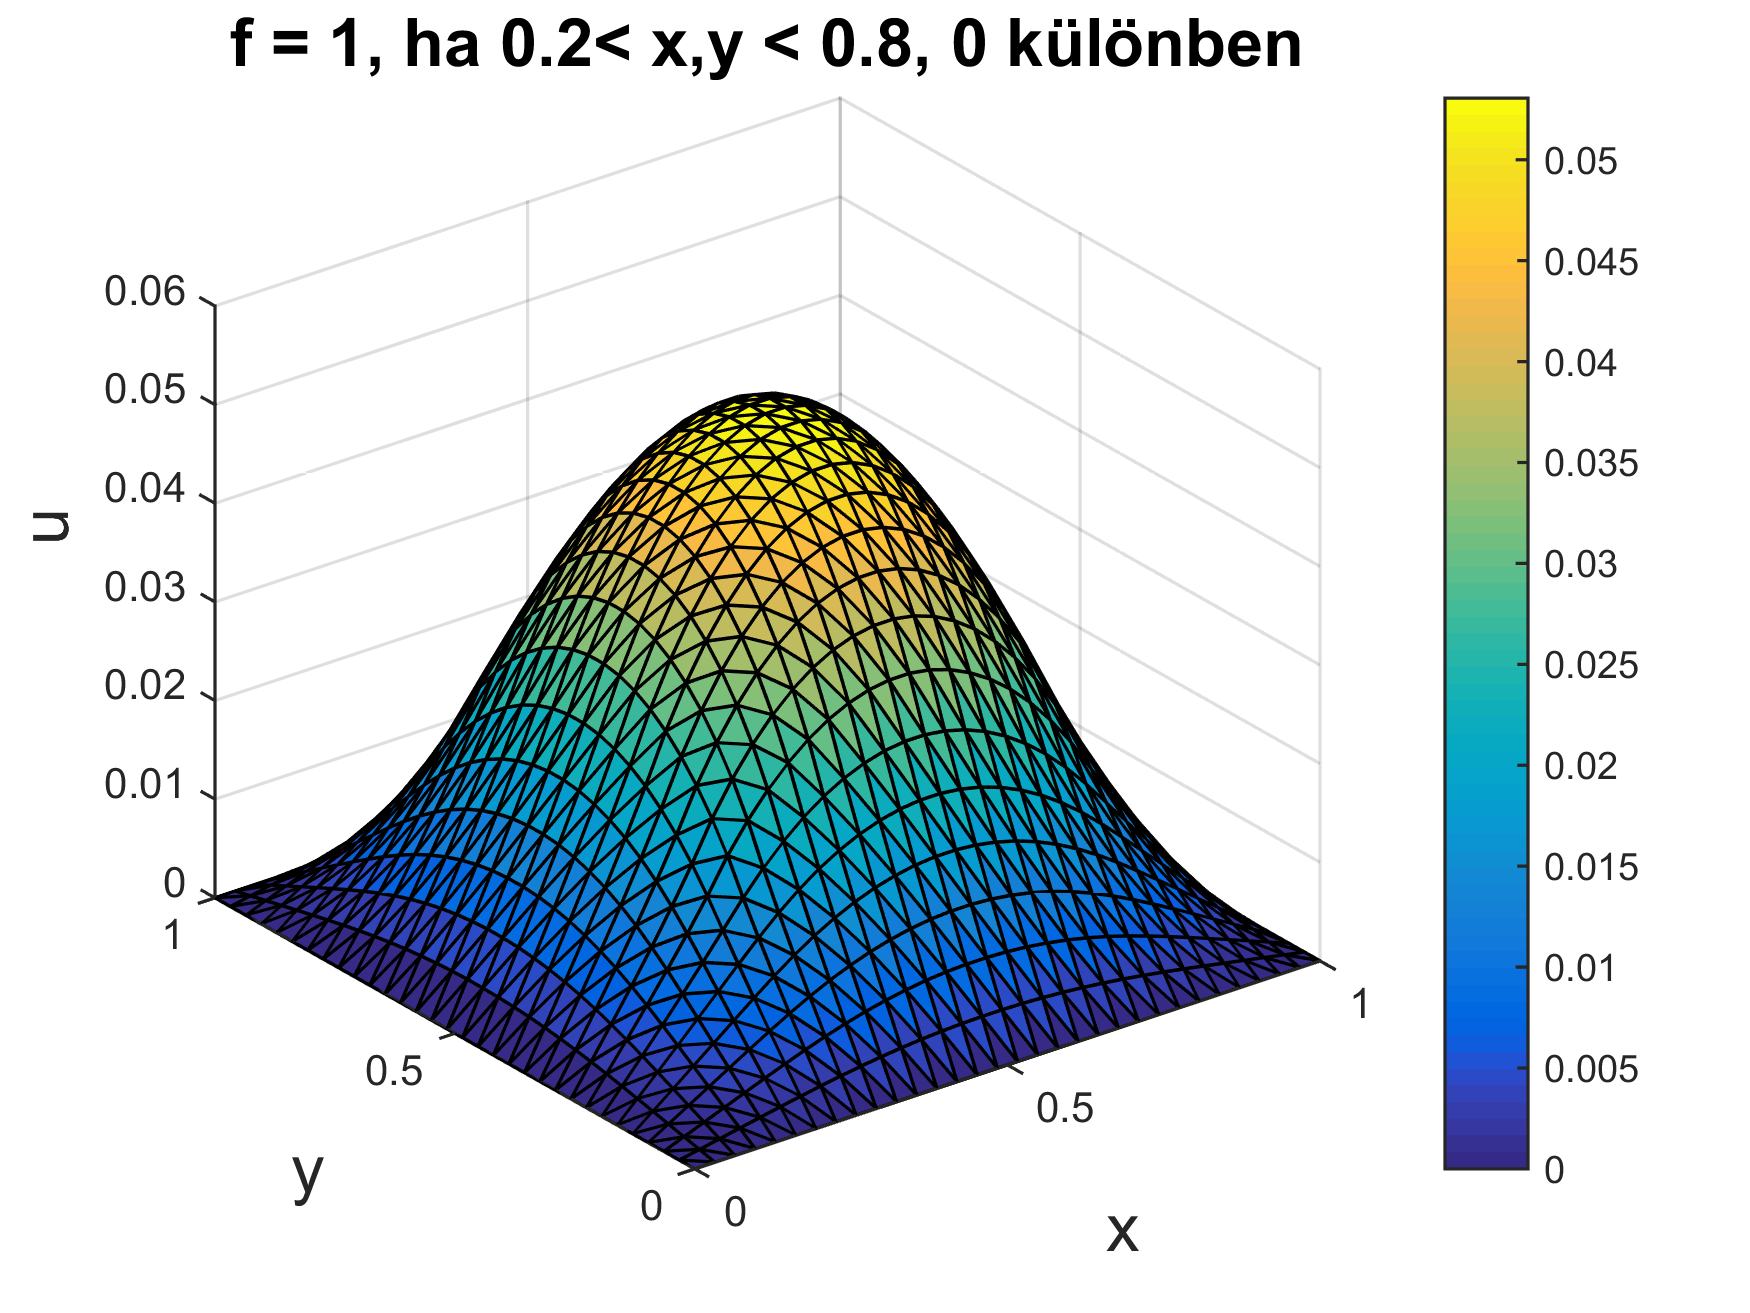
\includegraphics[width=\textwidth]{center20.png}}
		\label{fig:linu2d}
	\end{subfigure}
	\caption{Eredmények az $f_{3,k}$ és $f_{4,k}$ jobb oldali függvényekre \eqref{f_ek_szamitashoz}, $k = 1/3, 1/5$ mellett.}
	\label{fig:f34eredmeny}
\end{figure}


Az eredményekből látszik, hogy az $u_h$ végeselemes megoldás nemnegativitása mindegyik forrásfüggvény mellett teljesül. 

Az $f_{2,k}$ függvény esetében a forrás a jobb oldali $k$ szélességű sávon $1$, és a bal oldali $(1-k)$ szélességű sávon $0$. Az eredményekből látható (\ref{fig:f12eredmeny} ábra), hogy  kisebb $k$ értékek mellett a megoldás jobban megközelíti a $0$ értéket. A megoldás kovkáv felület, és kisebb $k$ értékek mellett az  $(1,y)$ szakaszon az $u_h$ gradiensvektora kisebb meredekségű.



Az $f_{3,k}$ és $f_{4,k}$ források esetében is teljesül, hogy ha a forrás kisebb területen $1$ és nagyobb részen $0$, akkor a megoldás közelebb van $0$-hoz  (\ref{fig:f34eredmeny} ábra). Az $f_{3,k}$ forráshoz tartozó megoldásoknál elmondható, hogy kisebb $k$-ra az $u_h$ a tartomány széléhez közelebb éri el maximumát. Az $f_{4,k}$ forrásra számított eredmények esetében pedig az látható, hogy kisebb $k$ értékek mellett a  széleken az $u_h$ gradiensvektora kisebb meredekségű.

